\documentclass{article}
\usepackage[spanish]{babel}
\usepackage[utf8]{inputenc}
\usepackage[letterpaper,top=2cm,bottom=2cm,left=3cm,right=3cm,marginparwidth=1.75cm]{geometry}
\usepackage{amsmath}
\usepackage[colorlinks=true, allcolors=blue]{hyperref}
\usepackage{makeidx}
\usepackage{fancyhdr}
\usepackage{xcolor}
\usepackage[document]{ragged2e}
\usepackage{imakeidx}
\usepackage{hyperref}
\usepackage{graphicx}
\usepackage{wrapfig}

\definecolor{rojo}{RGB}{255,0,0}
\definecolor{azul}{RGB}{12,0,200}

%Configurar el encabezado de pagina
\pagestyle{fancy}
\lhead{Análisis y Diseño de Sistemas}
\chead{}
\rhead{5CM4 - Análisis y Diseño de Sistemas}
\renewcommand{\headrulewidth}{0.4pt} % Ancho de la línea horizontal del encabezado

% Cargar el paquete makeidx para el índice
\makeindex

%\begin{document}
%Portada
\begin{document}
\begin{titlepage}
\centering
{\bfseries\LARGE Instituto Politécnico Nacional \par}
\vspace{.5cm}
{\bfseries\LARGE Escuela Superior de Computo \par}
\vspace{1cm}
\Large ANÁLISIS Y DISEÑO DE SISTEMAS \par
\vspace{1cm}
\itshape\LARGE Entregable Proyecto \par
\vspace{1cm}
%\itshape\LARGE Requerimientos funcionales, no funcionales y reglas de negocio \par
%\vspace{2cm}
\LARGE 5CM4\par
\vspace{1cm}

\begin{FlushLeft}
\Large Nombre del equipo: Bellakitos FC\par
\vspace{0.5cm}
\Large Profesora: Maldonado Castillo Idalia	 \par
\vspace{0.5cm}
    Integrantes:\\
    \begin{enumerate}
    \item Alvarado Díaz Dario\\
   \item Cervantes Maxtla Saúl\\
    \item Dominguez Olvera Leonardo Daniel\\
    \item Espinosa de los Monteros Martínez Eric Omar\\
   \item Estrada Yepez Omar Said\\
   \item García Torres Adair\\
   \item Ledesma Ramírez José Emiliano\\
   \item Murillo Mendoza María Fernanda\\
   \item Peña Ramírez Jonathan\\
   \item Ramírez Martínez Kevin Andrés\\
   \item Rojo Segura José Emmanuel\\
   \item Zamarrón Ramírez Javier\\
    \end{enumerate}
\vspace{.5cm}
\Large Fecha de Entrega: 2 de Octubre de 2023 \par
\vspace{.5cm}
\end{FlushLeft}
\end{titlepage}
\tableofcontents
\newpage
\section{Alcance del proyecto}
\justifying
Sistema que fomente el turismo el cual sera una aplicación movil, donde el turista que lo use se le mostrara en un mapa su ubicacion geografica a traves de su GPS y sea capaz de recomendarle sitios turisticos cercanos a su ubicacion para visitar de acuerdo a su medio de transporte ya sea caminando o utilizando un vehiculo. Los sitios turisticos deberan tener una clasificación como museos, restaurantes, parques entre otros sitios de interes. El sistema solo sera funcional a nivel nacional, es decir, solamente en México.

\section{Requerimientos Funcionales}
\subsection{Usuario Turista}
\begin{itemize}
    \item El sistema deberá acceder a la ubicación del usuario turista.
    \item El sistema debe permitir al usuario turista buscar lugares  en el mapa cercanos basados en su ubicación en un radio de 1 km a 10 km.
    \item El sistema debe permitir al usuario turista la creación de un perfil mediante un correo y una contraseña.
    \item El sistema debe permitir al usuario turista iniciar sesión.
    \item El sistema debe permitir al usuario turista cerrar sesión.
    \item El sistema debe permitir al usuario turista visualizar y modificar sus datos tales como nombre, correo, región, sitios de interés, radio de búsqueda y horarios y a su vez modificarlos en cualquier momento.
    \item El sistema deberá mostrar al perfil turista las reseñas de cada sitio de interés.
    \item El sistema permitirá al perfil turista crear itinerarios basándose en los horarios y cercanía de los sitios de interés.
    \item El sistema deberá permitir al perfil usuario turista guardar ubicaciones en favoritos.
    \item El sistema deberá generar una ruta basada en los lugares listados en el itinerario partiendo de la ubicación del perfil usuario turista.
    \item El sistema deberá permitir al usuario turista seleccionar su forma de desplazamiento.
    \item El sistema deberá permitir al usuario turista eliminar su cuenta.
    \item El sistema deberá mostrar información de los lugares señalados tales como su nombre, dirección, horarios, calificación, distancia y opciones de agregar itinerario, visitar y agregar a favoritos.
\end{itemize}

\subsection{Usuario Administrador}
\begin{itemize}
    \item El sistema deberá permitir al usuario administrador visualizar y actualizar los datos del usuario turista.
    \item El sistema deberá permitir al usuario administrador suspender y/o eliminar cuentas del usuario turista.
   \item El sistema deberá permitir al usuario administrador iniciar y cerrar sesión.
 \end{itemize}

\section{Requerimientos No Funcionales}
\begin{enumerate}
    \item Los datos de ubicación de los usuarios deberán ser tratados con privacidad de acuerdo a las políticas señaladas al momento de la creación de su cuenta por medio de un documento que las indique.
    
    \item El sistema debe solicitar al usuario turista permiso para utilizar su ubicación a través de una ventana emergente al momento de iniciaizar el sitema por primera vez.
    
    \item El sistema deberá dar acceso a los usuarios turista en un tiempo aproximado de 10 minutos como maximo.

\item El sistema debe permitir al usuario visualizar sus datos, al hacer clic en "mi perfil". La sección de datos
de la cuenta debe mostrar al usuario información detallada sobre su perfil.

\item El sistema permitira al ususario turista agregar los lugares mediante un boton \textbf{Agregar itinerario} que se muestra en el apartado detalles del lugar a la sección itinerario

\item El usuario debe poder elegir en que horarios llegara a cada uno de los lugares mostrados en la sección itinerario, mediante un boton "" el usuario debera seleccionar una hora del listado mostrado.El sistema ordenara el itinerario con base a las horas idicadas de menor mayor. El sistema debera validar que las horas indicadas, no fueran señaladas en otro lugar, si la hora ya fue utilizada previamente, el sistema debera mostrar un mensaje que indique que la hora ya fue utilizada. El usuario debe poder modificar los horarios de los lugares a visitar cuando lo desee.

\item El sistema permitira al usuario turista marcar como visitado el lugar en la sección itinerario, por medio de un boton "visitado", al ser presionado cambiara de color indicando que fue visitado.  

\item El usuario debe poder eliminar los lugar de su itinerario mediante el boton rojo de eliminacion o eliminar todo el itinerio con el boto "eliminar itinerario". EL sistema debera validar la eliminacion a traves de una confirmación del usuario turista mostrada en una ventana emergente que señalara "confirmo eliminacion" y "cancelar". Si se da click en confirmo eliminación, el sistema debera actualizar el itinerario. Si se da clik a cancelar, el sistema debera devolver al usuario a la sección itinerario.

\item El sistema debera generar una ruta a partir de los lugares de la sección itinerario, la generacion de ruta se da al seleccionar el boton "generar ruta" que aparecera en la sección itinerario. El sistema mostrara la ruta generada en una nueva pantalla que aparecera el mapa y los lugares indicados con su ubicacion y el orden que debera seguir visualizandose por lineas.

\item El sistema debera permitir mostrar los lugares en el mapa. El usuario debe poder dar click a los diferentes lugares, el sistema debera mostrar informacion del lugar y un boton que indique ver detalles del lugar seleccionado.

\item El sistema debera mostrar la informacion del lugar indicado a traves del boton "detalles". El usuario debe poder seleccionar agregar a itinerario, marcar como visitado y/o como favorito. El sistema debera agregar a favoritos, itinerario y/o visitado con base a la eleccion del usuario.

\item El usuario debe poder buscar diferentes lugares en los buscadores las secciones pantalla mapa, itinerario, historial y favoritos. EL sistema debera mostrar los lugares relacionados a la palabra colocada, Se debera ver la visualizacion de su nombre e imagen del lugar.

\item El sistema permitira la visualizacion de los lugares favoritos del usuario a traves de darle click a favoritos mostrado en la pantalla opciones. El usuario debe poder agregar y/o eliminar sus favoritos mediante los botones verde-agregar y rojo-eliminar. El sistema debera permitir buscar sus lugares favoritos mediante la opcion de busqueda.

\item El sistema permitira la visualizacion de su historial del usuario a traves de darle click en historial mostrado en la pantalla perfil. El sistema debera cambiar la pantalla a la sección historial. El usuario debe poder seleccionar ver detalles y eliminar historial completo. El sistema debera permitir buscar sus lugares visitado mediante la opcion de busqueda. El sistema debe poder eliminar toda la lista de historial mostrado con el boton "Eliminar historial", el sistema vaciara todo el historial.
    
    \item Los datos de los usuarios, como su informacion personal correo y contraseña, deben estar protegidos mediante cifrado y protección de dato.
    
    \item El sistema debe implementar mecanismos de autenticación y autorización sólidas para proteger los datos de los usuarios y garantizar que solo tengan acceso a su propia información, atraves de su nombre de usuario y correo electronico.

    \item El sistema debera verificar en la base de datos los correos electronicos, con la finalidad de que sean unicos para los usuarios turistas al momento del registro de una nueva cuenta. Los correos electronicos solo pueden ser utilizados una unica vez en una cuenta.

    \item El sistema deberá ser responsivo en dispositivos móviles con pantallas a partir de una resolución de 375x667 px hasta 820x1180.
    
    \item El sistema deberá ser responsivo en dispositivos de cómputo con pantallas de una resolución de 1280x720 px.
    
    \item El sistema debe ser capaz de integrarse con servicios de mapas y navegación para proporcionar direcciones y rutas precisas a partir de la API de Google.
    
    \item El sistema debe ser capaz de manejar al menos 20 usuarios concurrentes sin degradación significativa del rendimiento utilizando balanceadores de carga.
    
    \item La precisión de la ubicación debe ser lo más precisa posible, al menos 2 km, teniendo en cuenta las capacidades del hardware del dispositivo del usuario a través de la activación del GPS de dicho dispositivo.
    
    \item El sistema no deberá estar disponible únicamente en periodos de mantenimiento previamente señalados al usuario turista a traves de notificaciones por medio del sistema.
    
    \item El sistema deberá cerrar la sesión del usuario turista cuando él lo indique por medio de un botón visible que estara ubicado en la parte de sus datos de usuario. Al hacer clic en el botón, el sistema deberá cerrar la sesión de manera inmediata y redirigir al usuario turista a la página de inicio de sesión y debera recibir un mensaje de confirmación que indique que la sesión se ha cerrado de manera segura. 
    
    \item El sistema debe contar con medidas de seguridad para evitar un usuario pueda acceder a la cuenta de otro usuario mientras este abierta su sesión en un dispositivo que ha dejado su sesión abierta, por lo tanto solo se tendria una sesion iniciada en un unico dispositivo.
    

\item  El sistema permitira la recuperación de contraseña mediante la opcion "Olvidaste tu contraseña" en el apartado de iniciar sesion, mediante su correo electronico registrado previamente al momento de la creacion de su cuenta validando la información proporcionada por el usuario asegurándose de que los campos obligatorios estén completos y que la información proporcionada sea válida.El sistema también debe incluir medidas de seguridad para garantizar la protección de la información personal del usuario turista durante el proceso de recuperación de su contraseña.
\end{enumerate}

\section{Reglas de Negocio}
\begin{enumerate}
    \item \textbf{Registro de Usuarios}:
    \begin{itemize}
        \item Los usuarios turistas deben proporcionar un correo electrónico válido y una contraseña para registrarse en el sistema.
        \item El sistema no deberá permitir el registro de dos usuarios con la misma dirección de correo electrónico ni con el mismo nombre de usuario.
    \end{itemize}
    
    \item \textbf{Inicio de Sesión}:
    \begin{itemize}
        \item Los usuarios turistas deben iniciar sesión con su correo electrónico y contraseña registrados.
        \item El sistema debe verificar las credenciales del usuario antes de permitir el acceso.
    \end{itemize}
    
    \item \textbf{Acceso a la Ubicación}:
    \begin{itemize}
        \item El sistema debe obtener el consentimiento del usuario turista para acceder a su ubicación por medio de una ventana emergente cuando se abra por primera el sistema.
        \item El acceso a la ubicación debe ser desactivable por parte del usuario en cualquier momento.
    \end{itemize}
    
    \item \textbf{Búsqueda de Lugares Cercanos}:
    \begin{itemize}
        \item El usuario turista podrá filtrar la búsqueda seleccionando las categorías de su preferencia tales como restaurantes, parques, museos, entre otros.
        \item Los usuarios turistas pueden buscar lugares de interés dentro de un radio de 1 km a 10 km de su ubicación actual.
        \item Los resultados de la búsqueda deben basarse en la ubicación actual del usuario.
    \end{itemize}
    
    \item \textbf{Creación de Perfiles}:
    \begin{itemize}
        \item Los usuarios turistas pueden crear un perfil proporcionando un correo electrónico y contraseña válidos, además de un usuario único, así como sus datos personales como nombre, teléfono, edad y preferencias de lugares de interés.
        \item Las contraseñas deberán tener al menos una letra mayúscula y un carácter especial (*,@, -), tener una longitud mínima de 8 caracteres y máxima de 12, y utilizar caracteres alfanuméricos.
    \end{itemize}
    
    \item \textbf{Visualización/Modificación de Datos de Perfil}:
    \begin{itemize}
        \item Los usuarios turistas pueden ver y editar su nombre, región, sitios de interés, radio de búsqueda, contraseña.
        \item Los usuarios turistas solo visualizarán los datos de nombre de usuario y correo electrónico sin realizar modificaciones.
    \end{itemize}
    
    \item \textbf{Reseñas de Sitios de Interés}:
    \begin{itemize}
        \item Los usuarios turistas pueden ver reseñas de otros usuarios sobre lugares de interés.
        \item Solo los usuarios autenticados pueden dejar reseñas.
    \end{itemize}
    
    \item \textbf{Creación de Itinerarios}:
    \begin{itemize}
        \item Los usuarios turistas pueden crear itinerarios basados en la cercanía y horarios de los lugares de interés.
        \item Deben especificar la fecha y hora de inicio de cada itinerario.
    \end{itemize}
    
    \item \textbf{Guardado de Ubicaciones en Favoritos}:
    \begin{itemize}
        \item Los usuarios turistas pueden guardar lugares de interés en su lista de favoritos para acceder fácilmente en el futuro.
    \end{itemize}
    
    \item \textbf{Selección de Forma de Desplazamiento}:
    \begin{itemize}
        \item Los usuarios turistas pueden elegir su forma de desplazamiento preferida, como caminar, conducir, o usar transporte público (PENDIENTE).
    \end{itemize}
    
    \item \textbf{Privacidad de Datos}:
    \begin{itemize}
        \item Los usuarios turistas deberán aceptar los términos y condiciones mostrados al momento de crear una cuenta.
        \item Los datos personales de los usuarios, como el correo electrónico y la ubicación, deben mantenerse confidenciales y protegerse de acuerdo con las regulaciones de privacidad aplicables (CUALES).
    \end{itemize}
    
    \item \textbf{Borrado de Cuentas}:
    \begin{itemize}
        \item Los usuarios turistas pueden eliminar sus cuentas de usuario si lo desean, lo que resultará en la eliminación permanente de sus datos.
    \end{itemize}
\end{enumerate}

%ARCHIVO DE DIAGRAMAS
\section{Diagrama de Casos de Uso}
    \begin{figure}[htbp]
        \centering
        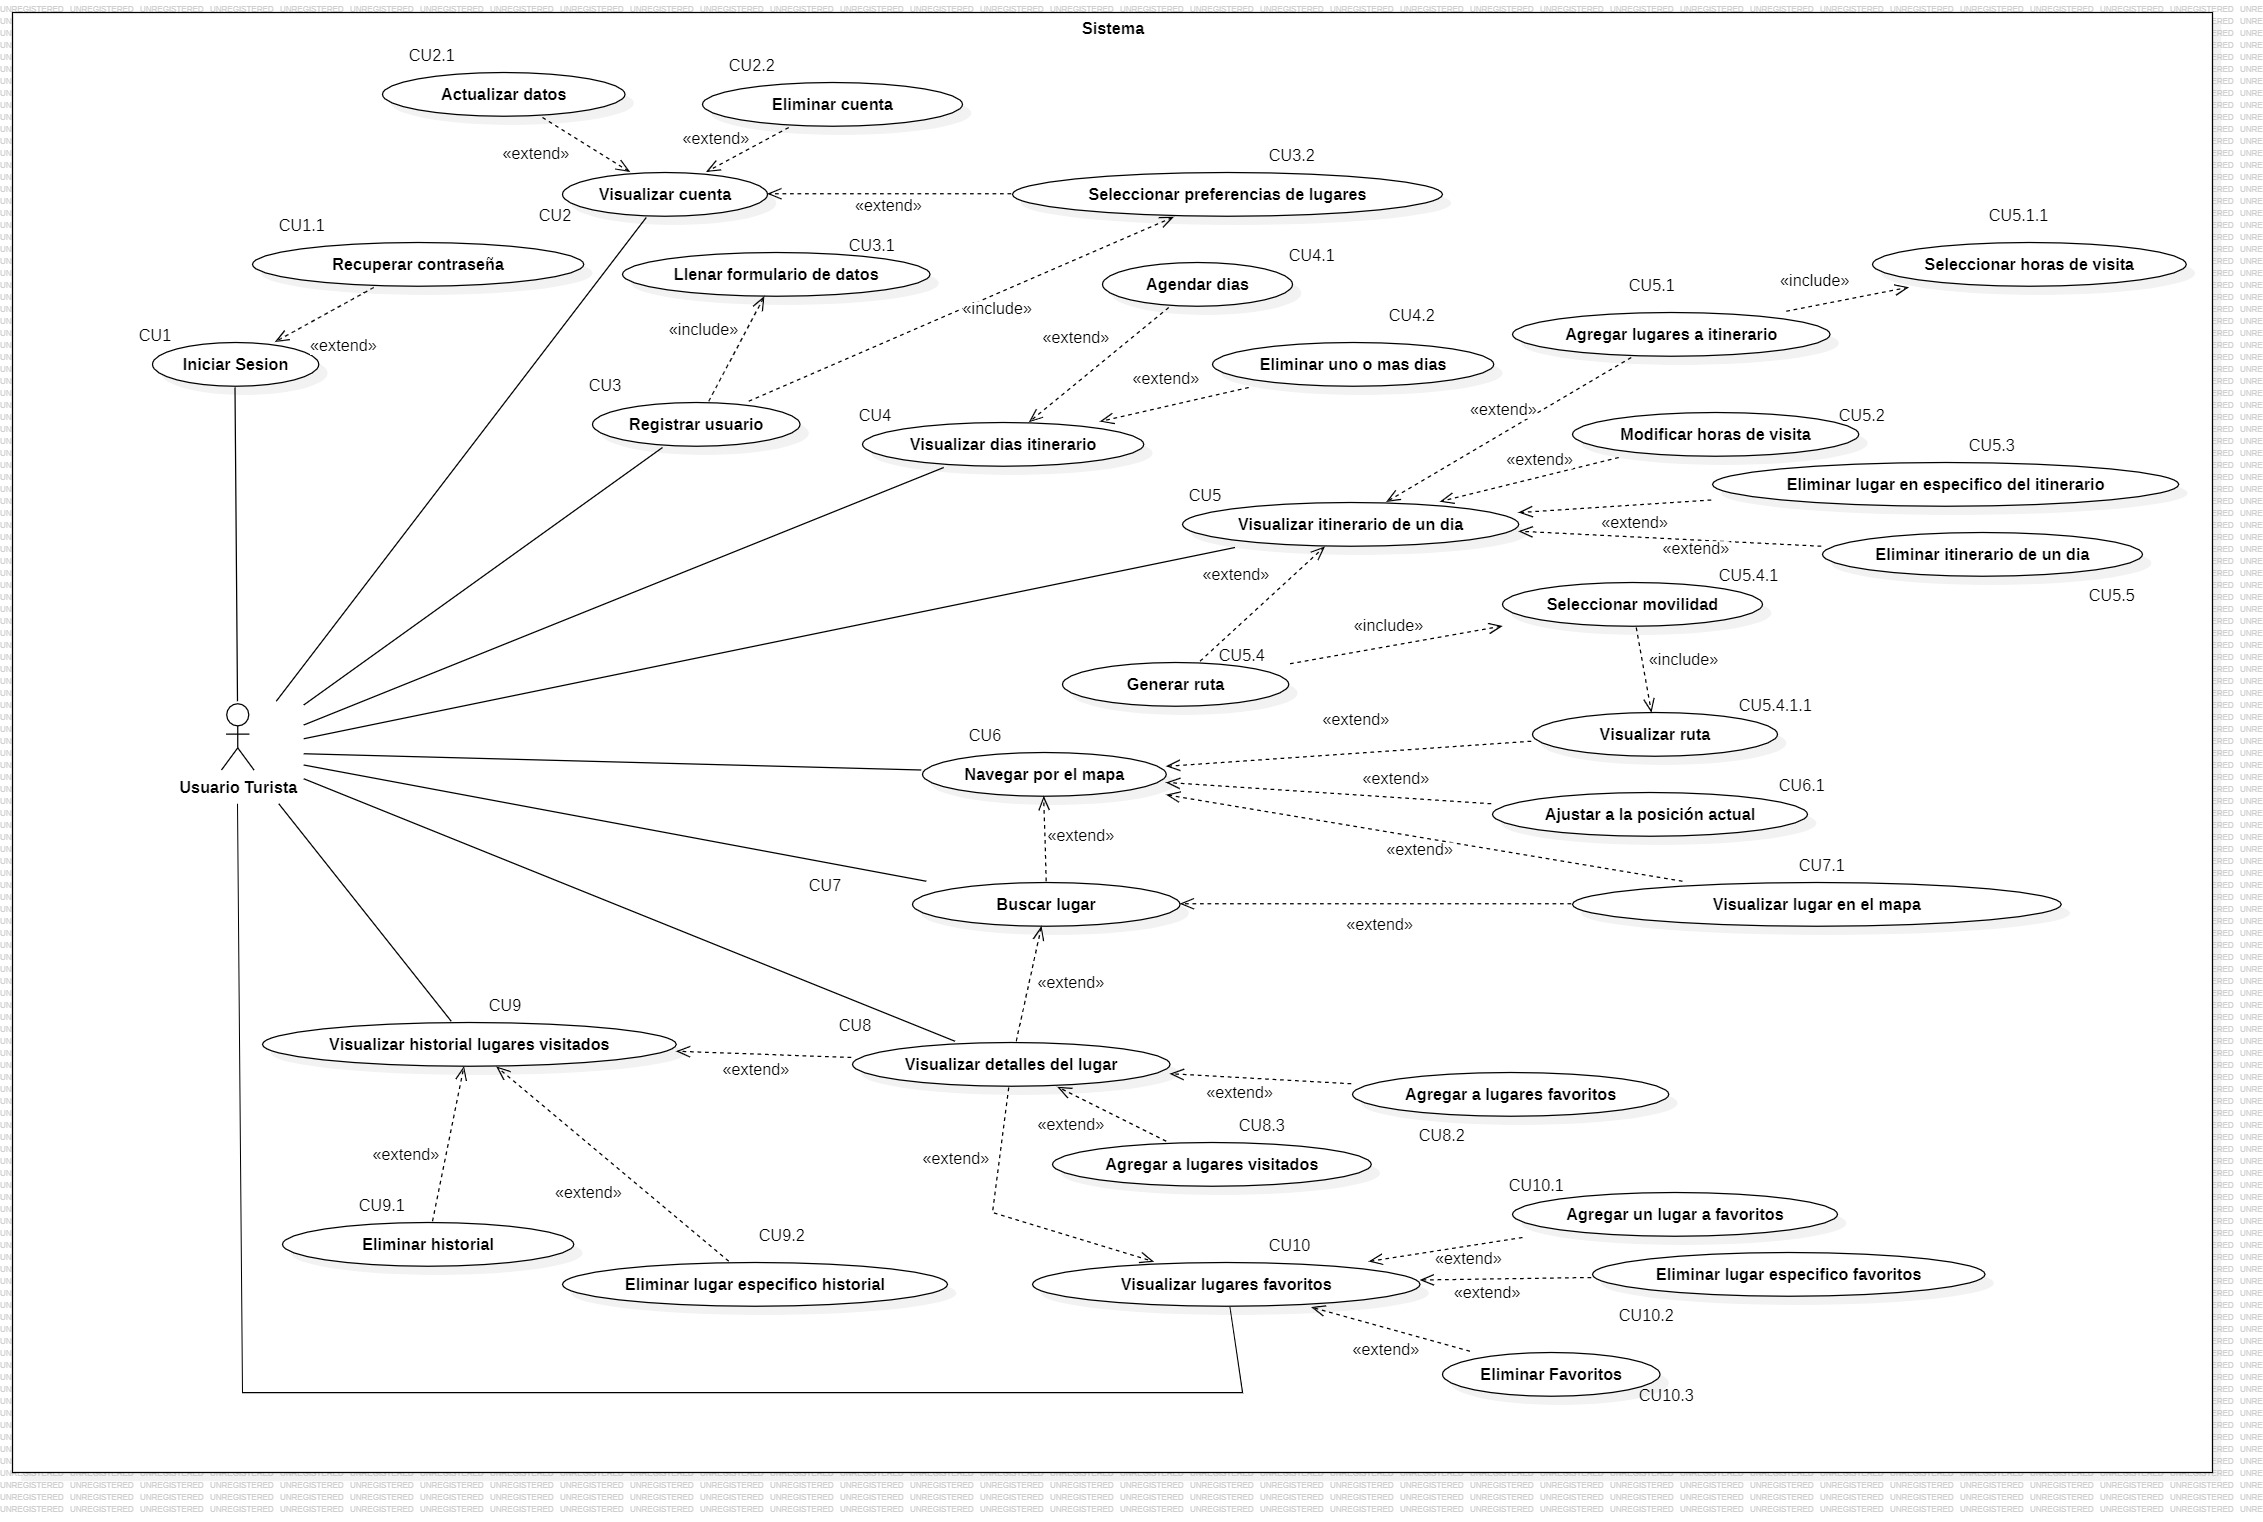
\includegraphics[width=16.5cm]{entregable final/caso_usoSA.jpg}
        \caption{Diagrama de Caso de Uso}
        \label{fig:enter-label}
    \end{figure}
    
\section{\textcolor{azul}{Definición de actores propuestos}}
\textbf{Usuario Admin}\\
Es el usuario que gestionara  el sistema cuyas principales funciones son getsionar y suspendercuentas de los turistas.\\
\vspace{.5cm}
\textbf{Usuario Turista}\\
Es el usuario que interactua con el sistema, es decir, el cliente de nuestra aplicacion, sus principales caracteristicas son creacion de cuentas para poder acceder al sistema, iniciar sesión en el sistema, visualizar su ubicacion en un mapa, poder visualizar sus datos de usuario, generar un itinerario de su ruta turistica, contar con un historial de los sitios que ha visitado, poder tener un apartado de favoritos, cerrar sesión, organizar sus horarios. 

%ARCHIVO DE PANTALLAS
\section{\textcolor{azul}{Prototipo no funcional}}
%jony
\begin{figure}[h]
    \begin{minipage}{0.4\textwidth}
        \centering
        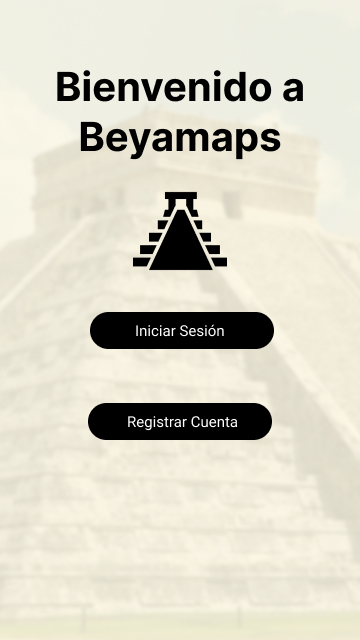
\includegraphics[width=.7\linewidth]{Pantallas Prototipo3/IU01 Pantalla incial.jpg}
        \caption{IU01 Pantalla incial}
    \end{minipage}
    
    \begin{minipage}{0.4\textwidth}
        \centering
        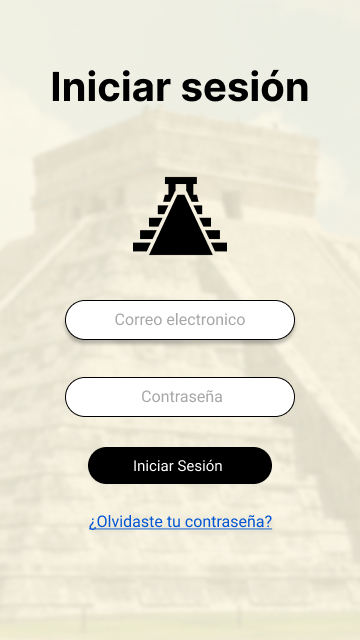
\includegraphics[width=.7\linewidth]{Pantallas Prototipo3/IU02 Pantalla Iniciar sesion.jpg}
        \caption{IU02 Pantalla Iniciar sesion}
    \end{minipage}%
\end{figure}

\begin{figure}[h]
    \begin{minipage}{0.5\textwidth}
        \centering
        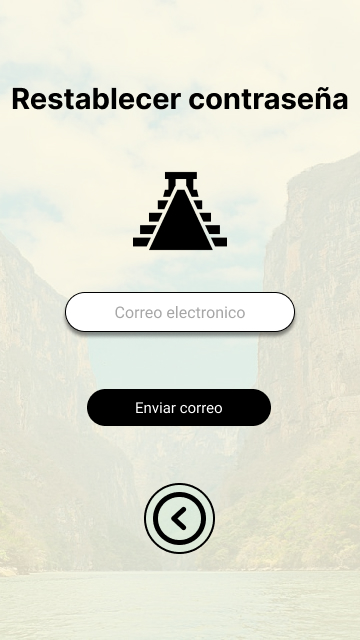
\includegraphics[width=.7\linewidth]{Pantallas Prototipo3/IU03 Pantalla correo restablecimiento.jpg}
        \caption{IU03 Pantalla correo restablecimiento.}
    \end{minipage}
    
    \begin{minipage}{0.5\textwidth}
        \centering
        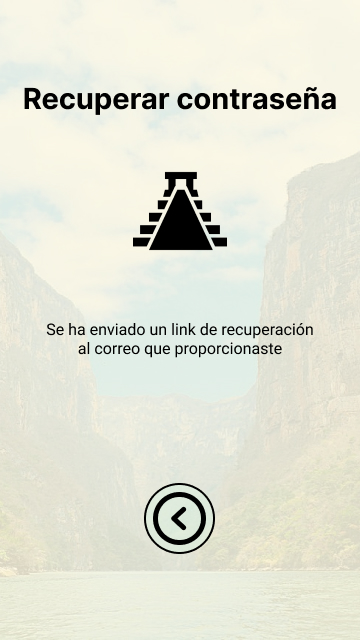
\includegraphics[width=.7\linewidth]{Pantallas Prototipo3/IU04 Pantalla link de recuperacion.jpg}
        \caption{IU04 Pantalla link de recuperacion}
    \end{minipage}%
\end{figure}

\begin{figure}[h]
    \begin{minipage}{0.5\textwidth}
        \centering
        \includegraphics[width=.7\linewidth]{Pantallas Prototipo3/IU05-Reestablacer contraseña.jpg}
        \caption{IU05 Reestablacer contraseña}
    \end{minipage}
    
    \begin{minipage}{0.5\textwidth}
        \centering
        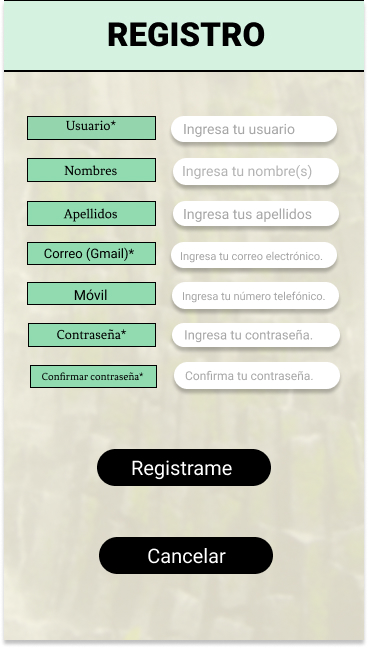
\includegraphics[width=.7\linewidth]{Pantallas Prototipo3/IU06-Registro de Cuenta.jpg}
        \caption{IU06 Registro de Cuenta}
    \end{minipage}%
\end{figure}

\begin{figure}[h]
    \begin{minipage}{0.5\textwidth}
        \centering
        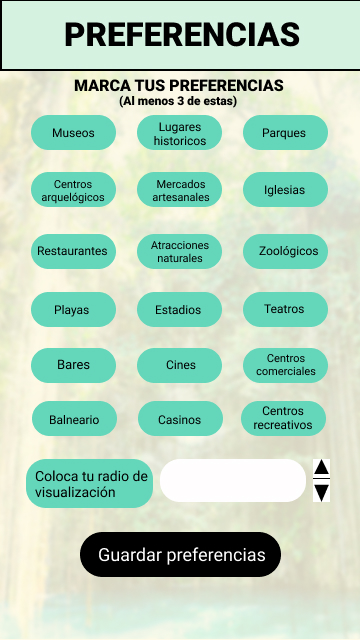
\includegraphics[width=.7\linewidth]{Pantallas Prototipo3/IU07-Preferencias del usuario.jpg}
        \caption{IU07 Preferencias del usuario}
    \end{minipage}
    
    \begin{minipage}{0.5\textwidth}
        \centering
        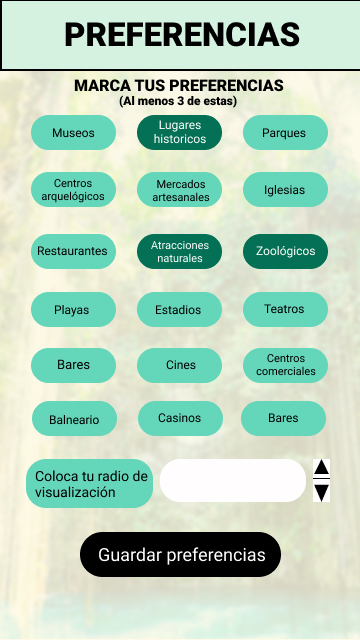
\includegraphics[width=.7\linewidth]{Pantallas Prototipo3/IU08-Preferencias del usuario.jpg}
        \caption{IU08 Preferencias del usuario seleccionadas}
    \end{minipage}%
\end{figure}

\begin{figure}[h]
    \begin{minipage}{0.5\textwidth}
        \centering
        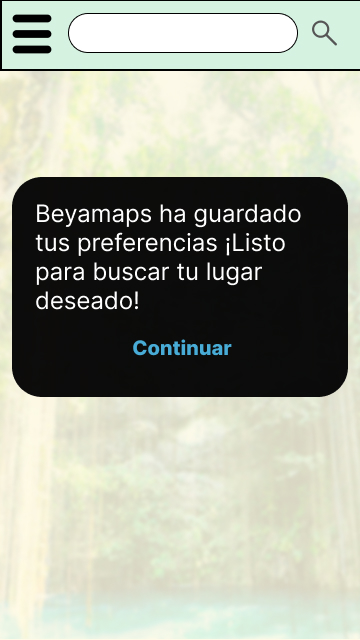
\includegraphics[width=.7\linewidth]{Pantallas Prototipo3/IU09Preferencias del usuario.jpg}
        \caption{IU09 Preferencias guardadas}
    \end{minipage}
    
    \begin{minipage}{0.5\textwidth}
        \centering
        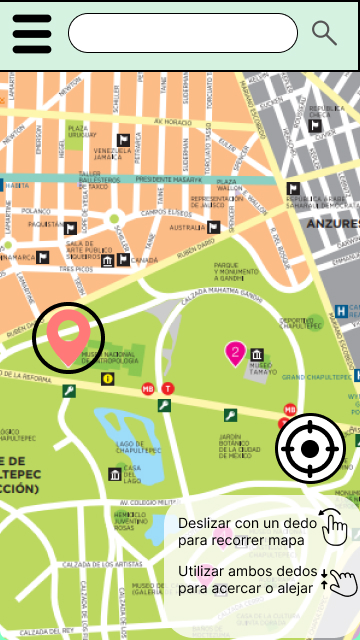
\includegraphics[width=.7\linewidth]{Pantallas Prototipo3/IU10 - Mapa principal.jpg}
        \caption{IU10 Mapa principal}
    \end{minipage}%
\end{figure}

\begin{figure}[h]
    \begin{minipage}{0.5\textwidth}
        \centering
        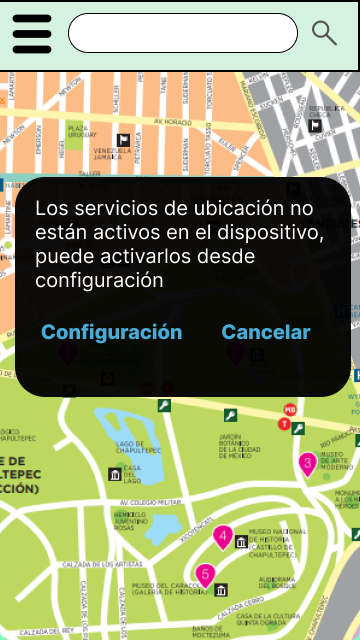
\includegraphics[width=.7\linewidth]{Pantallas Prototipo3/IU11 - Activar ubicacion.jpg}
        \caption{IU11 Activar ubicacion}
    \end{minipage}
%fin jony
%inicio Dario
    \begin{minipage}{0.5\textwidth}
        \centering
        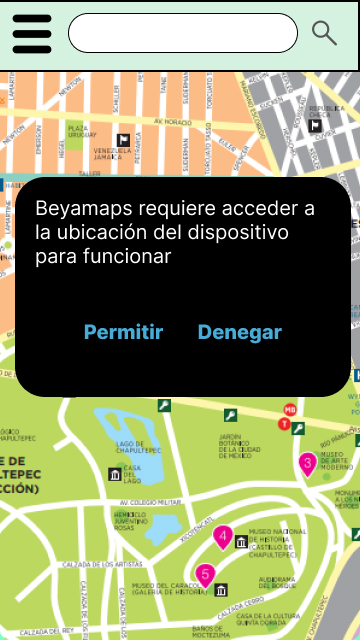
\includegraphics[width=.7\linewidth]{Pantallas Prototipo3/IU12 Pantalla Acceso Ubicacion.jpg}
        \caption{IU 12 Pantalla Acceso Ubicación}
    \end{minipage}%
\end{figure}

\begin{figure}[h]
    \begin{minipage}{0.5\textwidth}
        \centering
        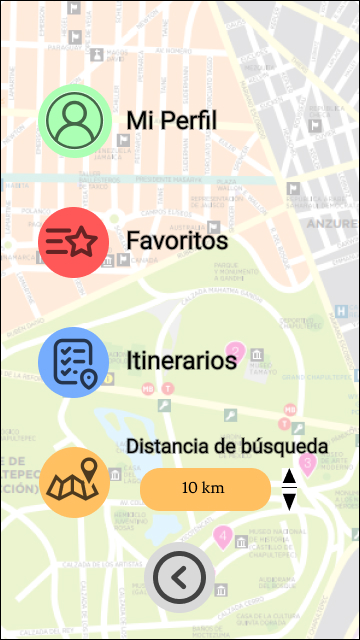
\includegraphics[width=.7\linewidth]{Pantallas Prototipo3/IU13 Pantalla Menu de Opciones.jpg}
        \caption{IU13 Pantalla Menu de Opciones}
    \end{minipage}
    
    \begin{minipage}{0.5\textwidth}
        \centering
        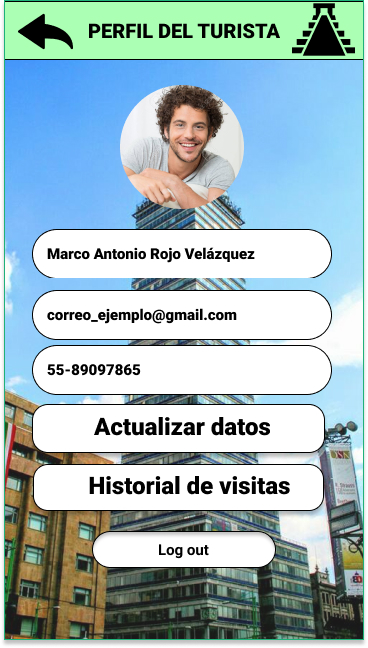
\includegraphics[width=.7\linewidth]{Pantallas Prototipo3/IU14 Pantalla de perfil.jpg}
        \caption{IU14 Pantalla Perfil}
    \end{minipage}%
\end{figure}

\begin{figure}[h]
    \begin{minipage}{0.5\textwidth}
        \centering
        \includegraphics[width=.7\linewidth]{Pantallas Prototipo3/IU15 Pantalla Validacion de Contraseña.jpg}
        \caption{IU15 Pantalla Validación de Contraseña}
    \end{minipage}
    
    \begin{minipage}{0.5\textwidth}
        \centering
        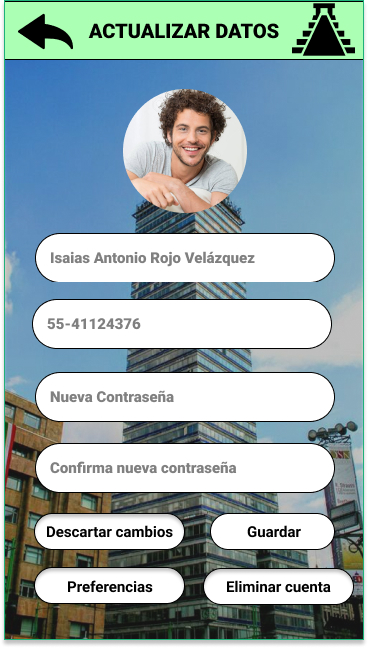
\includegraphics[width=.7\linewidth]{Pantallas Prototipo3/IU16 Pantalla de seleccionar el dato a editar.jpg}
        \caption{IU16 Pantalla Seleccionar Datos a Editar}
    \end{minipage}%
\end{figure}

\begin{figure}[h]
    \begin{minipage}{0.5\textwidth}
        \centering
        \includegraphics[width=.7\linewidth]{Pantallas Prototipo3/IU17 Pantalla Confirmación de guardado.jpg}
        \caption{IU17 Pantalla Confirmación de Guardado}
    \end{minipage}
    
    \begin{minipage}{0.5\textwidth}
        \centering
        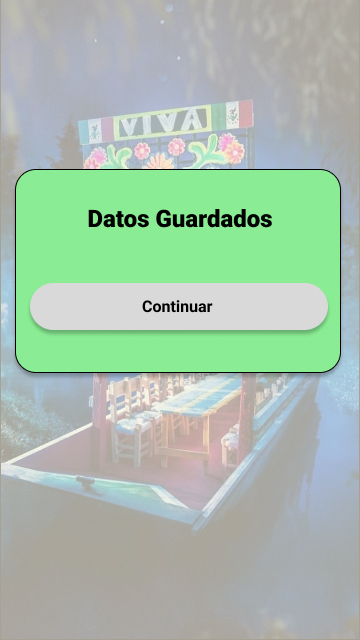
\includegraphics[width=.7\linewidth]{Pantallas Prototipo3/IU18 Pantalla Datos Guardados.jpg}
        \caption{IU18 Pantalla Datos Guardados}
    \end{minipage}%
\end{figure}

\begin{figure}[h]
    \begin{minipage}{0.5\textwidth}
        \centering
        \includegraphics[width=.7\linewidth]{Pantallas Prototipo3/IU19 Pantalla Ventana de confirmación de eliminar cuenta.jpg}
        \caption{IU19 Pantalla Ventana Confirmación Eliminar Cuenta}
    \end{minipage}
    
    \begin{minipage}{0.5\textwidth}
        \centering
        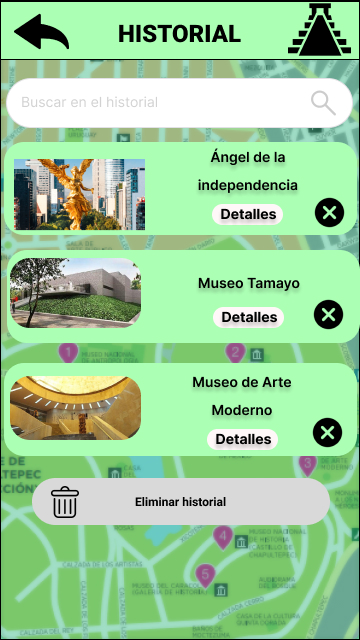
\includegraphics[width=.7\linewidth]{Pantallas Prototipo3/IU20 Pantalla Historial.jpg}
        \caption{IU20 Pantalla Historial}
    \end{minipage}%
\end{figure}

\begin{figure}[h]
    \begin{minipage}{0.5\textwidth}
        \centering
        \includegraphics[width=.7\linewidth]{Pantallas Prototipo3/IU21 Ventana confirmación eliminar.jpg}
        \caption{IU21 Pantalla Ventana Confirmación Eliminar}
    \end{minipage}
    
    \begin{minipage}{0.5\textwidth}
        \centering
        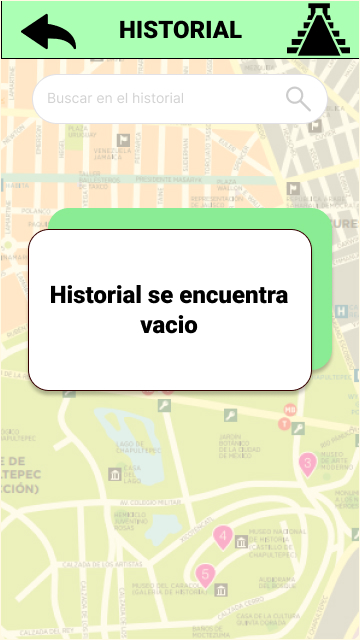
\includegraphics[width=.7\linewidth]{Pantallas Prototipo3/IU22 Historial vacio.jpg}
        \caption{IU22 Pantalla Historial Vacio}
    \end{minipage}%
\end{figure}
%fin dario
%inicio leo
\begin{figure}[h]
    \begin{minipage}{0.5\textwidth}
        \centering
        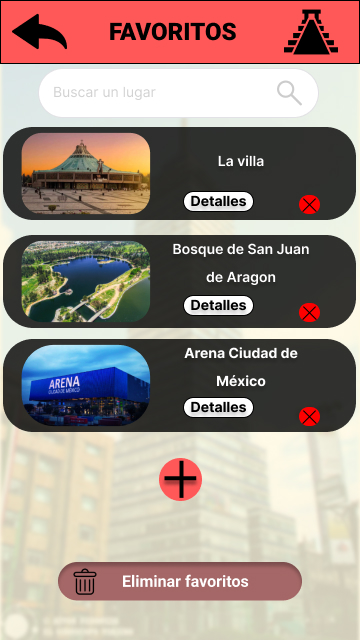
\includegraphics[width=.7\linewidth]{Pantallas Prototipo3/IU23 Pantalla Favoritos.jpg}
        \caption{IU23 Pantalla Favoritos}
    \end{minipage}
    
    \begin{minipage}{0.5\textwidth}
        \centering
        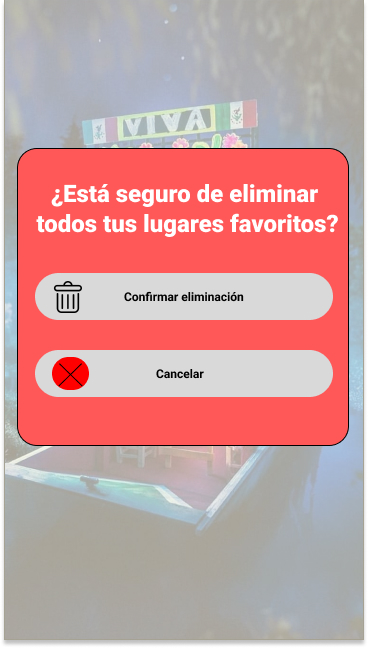
\includegraphics[width=.7\linewidth]{Pantallas Prototipo3/IU24 Pantalla Eliminacion favoritos.jpg}
        \caption{IU24 Pantalla Eliminacion favoritos}
    \end{minipage}%
\end{figure}

\begin{figure}[h]
    \begin{minipage}{0.5\textwidth}
        \centering
        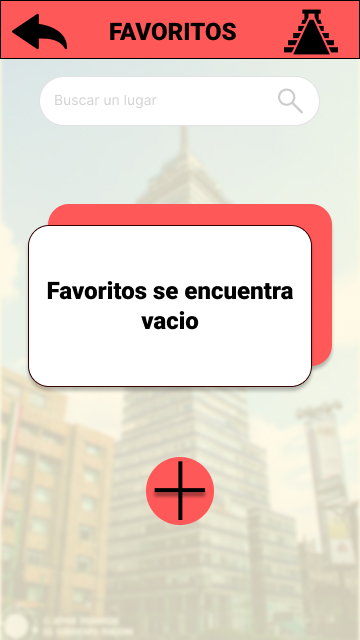
\includegraphics[width=.7\linewidth]{Pantallas Prototipo3/IU25 Pantalla Favoritos vacio.jpg}
        \caption{IU25 Pantalla Favoritos vacio}
    \end{minipage}
    
    \begin{minipage}{0.5\textwidth}
        \centering
        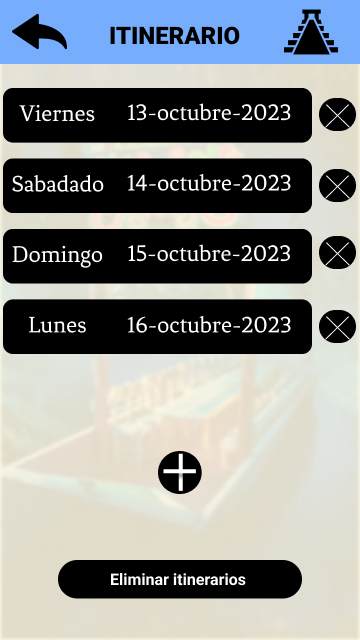
\includegraphics[width=.7\linewidth]{Pantallas Prototipo3/IU26 Pantalla Dias Itinerario.jpg}
        \caption{IU26 Pantalla Dias Itinerario}
    \end{minipage}%
\end{figure}

\begin{figure}[h]
    \begin{minipage}{0.5\textwidth}
        \centeringz
        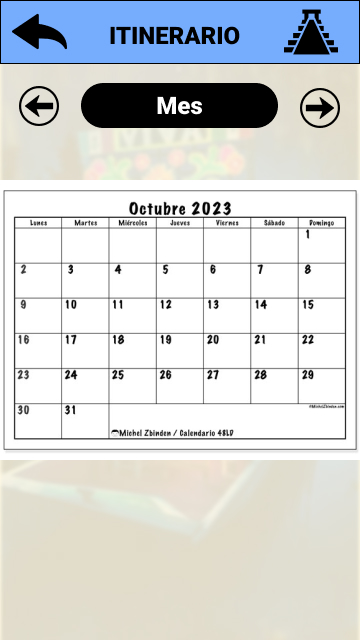
\includegraphics[width=.7\linewidth]{Pantallas Prototipo3/IU27 Pantalla Dia calendario.jpg}
        \caption{IU27 Pantalla Dia calendario}
    \end{minipage}
    
    \begin{minipage}{0.5\textwidth}
        \centering
        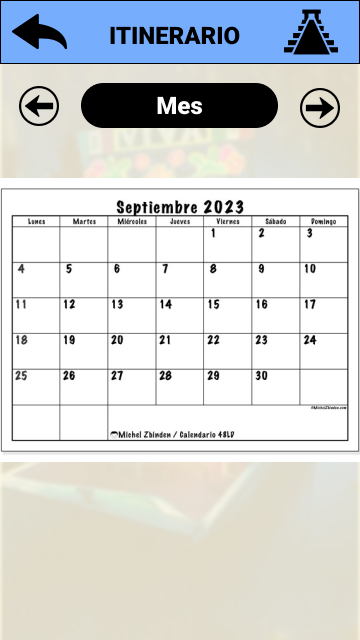
\includegraphics[width=.7\linewidth]{Pantallas Prototipo3/IU28 Pantalla Dia Mes Diferente.jpg}
        \caption{IU28 Pantalla Dia Mes Diferente}
    \end{minipage}%
\end{figure}

\begin{figure}[h]
    \begin{minipage}{0.5\textwidth}
        \centering
        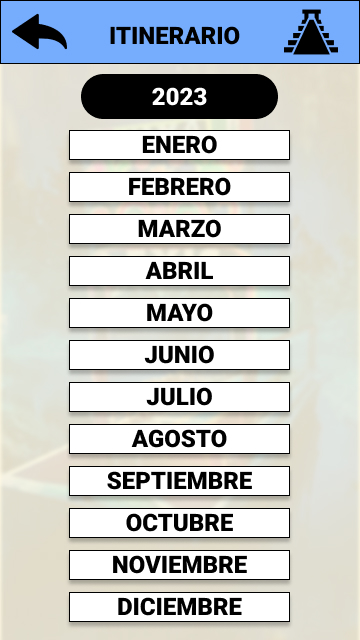
\includegraphics[width=.7\linewidth]{Pantallas Prototipo3/IU29 Pantalla Mes Calendario.jpg}
        \caption{IU29 Pantalla Mes Calendario}
    \end{minipage}
    
    \begin{minipage}{0.5\textwidth}
        \centering
        \includegraphics[width=.7\linewidth]{Pantallas Prototipo3/IU30 Pantalla Año Calendario.jpg}
        \caption{IU30 Pantalla Año Calendario}
    \end{minipage}%
\end{figure}

\begin{figure}[h]
    \begin{minipage}{0.5\textwidth}
        \centering
        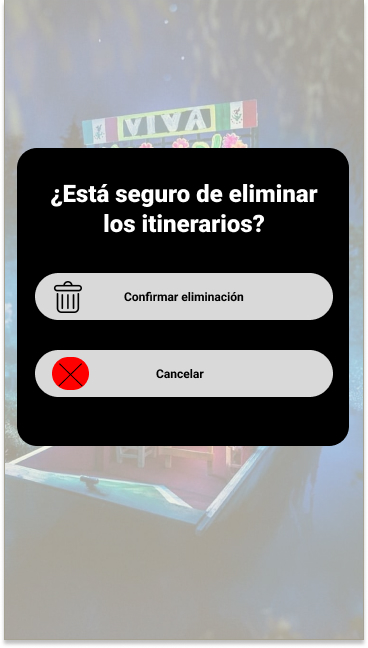
\includegraphics[width=.7\linewidth]{Pantallas Prototipo3/IU31 Pantalla Eliminar Itinerario.jpg}
        \caption{IU31 Pantalla Eliminar Itinerario}
    \end{minipage}
    
    \begin{minipage}{0.5\textwidth}
        \centering
        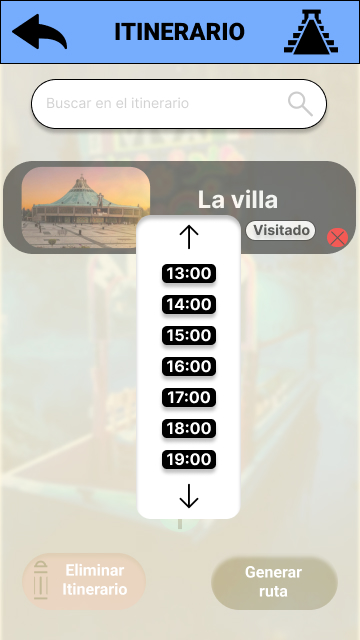
\includegraphics[width=.7\linewidth]{Pantallas Prototipo3/IU32 Pantalla Horas Lugar.jpg}
        \caption{IU32 Pantalla Horas Lugar}
    \end{minipage}%
\end{figure}

\begin{figure}[h]
    \begin{minipage}{0.5\textwidth}
        \centering
        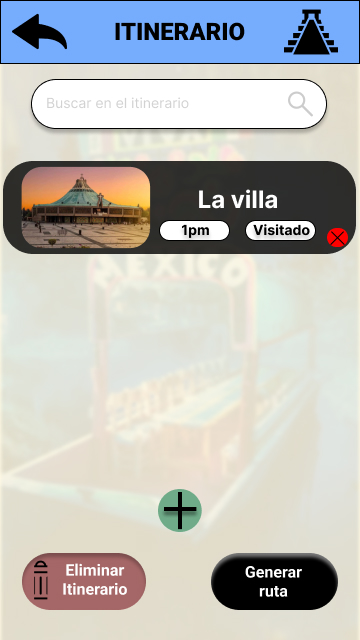
\includegraphics[width=.7\linewidth]{Pantallas Prototipo3/IU33 Pantalla Itinerario Dia.jpg}
        \caption{IU33 Pantalla Itinerario Dia}
    \end{minipage}
%fin leo
%inicio said
    \begin{minipage}{0.5\textwidth}
        \centering
        \includegraphics[width=.7\linewidth]{Pantallas Prototipo3/IU34-Ventana confirmación eliminar itinerario.jpg}
        \caption{IU34 Pantalla confirmación eliminar itinerario}
    \end{minipage}%
\end{figure}

\begin{figure}[h]
    \begin{minipage}{0.5\textwidth}
        \centering
        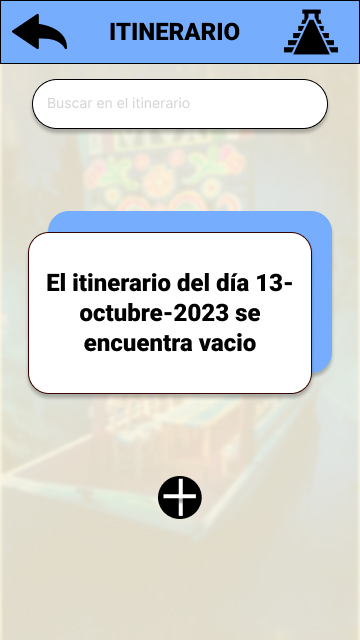
\includegraphics[width=.7\linewidth]{Pantallas Prototipo3/IU35-itinerario vacio en el dia x-x-x.jpg}
        \caption{IU35 Pantalla itinerario vacio en el dia x-x-x}
    \end{minipage}
    
    \begin{minipage}{0.5\textwidth}
        \centering
        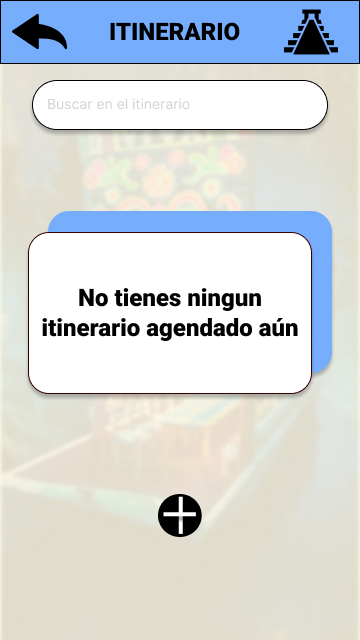
\includegraphics[width=.7\linewidth]{Pantallas Prototipo3/IU36-dias del itineraio vacio.jpg}
        \caption{IU36 Pantalla dias del itineraio vacio}
    \end{minipage}%
\end{figure}

\begin{figure}[h]
    \begin{minipage}{0.5\textwidth}
        \centering
        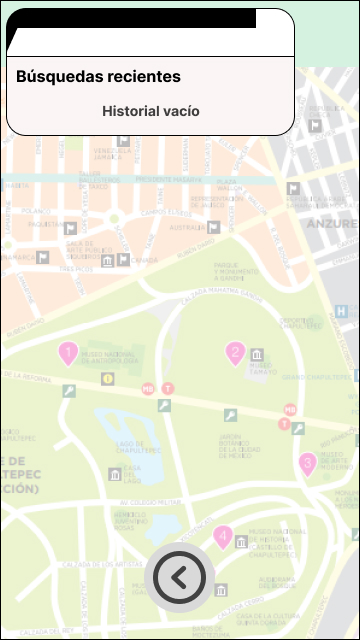
\includegraphics[width=.7\linewidth]{Pantallas Prototipo3/IU37-Historial de Búsqueda Vacío.jpg}
        \caption{IU37 Pantalla Historial de Búsqueda Vacío}
    \end{minipage}
    
    \begin{minipage}{0.5\textwidth}
        \centering
        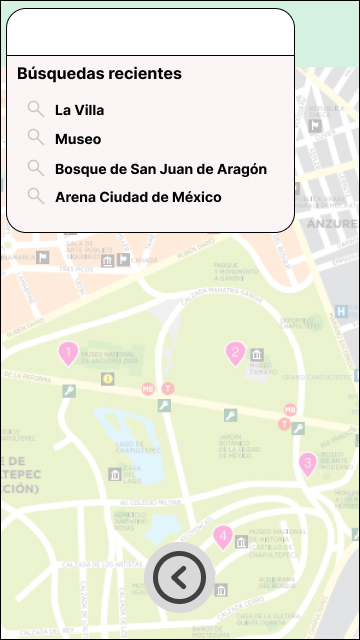
\includegraphics[width=.7\linewidth]{Pantallas Prototipo3/IU38-Buscar un lugar.jpg}
        \caption{IU38 Pantalla Buscar un lugar}
    \end{minipage}%
\end{figure}

\begin{figure}[h]
    \begin{minipage}{0.5\textwidth}
        \centering
        \includegraphics[width=.7\linewidth]{Pantallas Prototipo3/IU39-Búsqueda de un lugar.jpg}
        \caption{IU39 Pantalla Búsqueda de un lugar}
    \end{minipage}
    
    \begin{minipage}{0.5\textwidth}
        \centering
        \includegraphics[width=.7\linewidth]{Pantallas Prototipo3/IU40-Búsqueda sin resultado.jpg}
        \caption{IU40 Pantalla Búsqueda sin resultado}
    \end{minipage}%
\end{figure}

\begin{figure}[h]
    \begin{minipage}{0.5\textwidth}
        \centering
        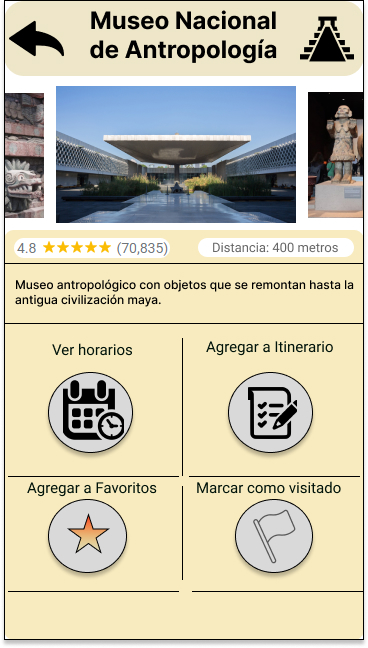
\includegraphics[width=.7\linewidth]{Pantallas Prototipo3/IU41-Detalles del lugar.jpg}
        \caption{IU41 Pantalla Detalles del lugar}
    \end{minipage}
    
    \begin{minipage}{0.5\textwidth}
        \centering
        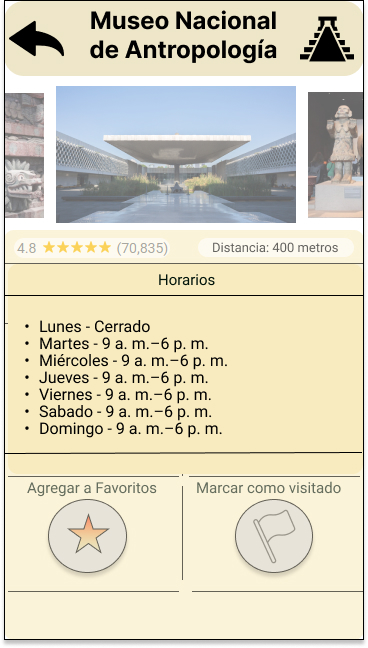
\includegraphics[width=.7\linewidth]{Pantallas Prototipo3/IU42-Ver horario.jpg}
        \caption{IU42 Pantalla Ver horario}
    \end{minipage}%
\end{figure}

\begin{figure}[h]
    \begin{minipage}{0.5\textwidth}
        \centering
        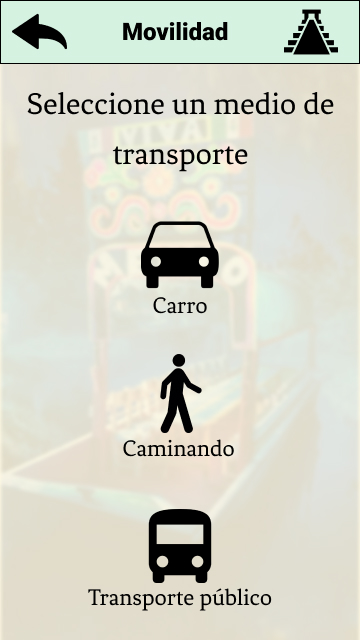
\includegraphics[width=.7\linewidth]{Pantallas Prototipo3/IU43-Movilidad.jpg}
        \caption{IU43 Pantalla Movilidad}
    \end{minipage}
    
    \begin{minipage}{0.5\textwidth}
        \centering
        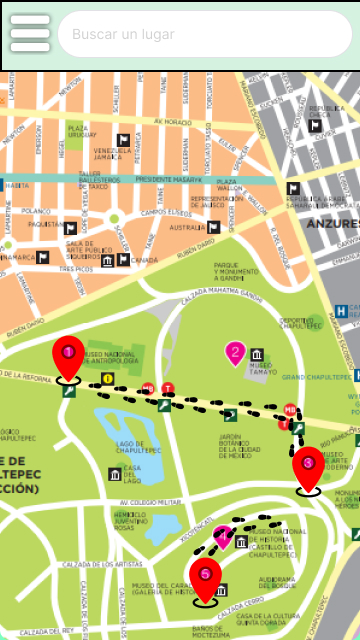
\includegraphics[width=.7\linewidth]{Pantallas Prototipo3/IU44-Ruta generada.jpg}
        \caption{IU44 Pantalla Ruta generada}
    \end{minipage}%
\end{figure}

\newpage


%\section{\textcolor{azul}{Referencias bibliográficas}}
%\begin{thebibliography}{99}
 %   \bibitem{ref1} 
   % \bibitem{ref2} 
  %  \bibitem{ref3} 
  %  \bibitem{ref4} 
  %  \bibitem{ref5} 
%\end{thebibliography}

% Imprimir el índice
\printindex

\end{document}